\scanpage{79}
I denote by $\widehat M^*_{\underline G,\underline G'}$, $\overset{\unsure{\deleted{\wedge}}}{M}{}^*_{\underline G,\underline G'}$ the germs of multiplicities obtained by \deleted{removing (``\unsure{infinity|the core}'') $\widehat M_{\underline G}$ resp. $M_{\underline G}$, $\unsure{\Gamma^!_{\underline G,\underline G'}}$ (the traces \unsure{of the union|on the germ} of the divisors of $\unsure{\widehat M_{\underline G'}}$ \unsure{that contain} $\unsure{(\widehat M_{\underline G},\Gamma^!_{G,G'})}$)}
\inserted{\deleted{\unsure{taking the traces of} $M$} removing the traces of the divisors at infinity of $\widehat M_{\underline G'}$ \deleted{\unsure{not alone}} that contain $\widehat M_{\unsure{\underline G|G}}$ -- in the case of $M^*_{\underline G,\underline G'}$, one takes the \uline{trace} of $M_{\underline G'}$ on $\widehat M_{\underline G,\underline G'}$}
\unsure{They are therefore} filters of open sets of the multiplicity $M_{G'}$, and the fundamental groupoids* \deleted{$\unsure{\Pi}$}
\[
(100)\qquad\Pi M^{\unsure{*|\leftarrow}}_{\underline G,\underline G'},\qquad\Pi M^{\unsure{*|\leftarrow}}_{\underline G,\underline G'}
\]
are defined as Categories $\underset{\longrightarrow}{\lim}$ of the categories of universal coverings, \unsure{or} or as categories of the coverings \unsure{of the connected} of the said germs of multi-plicities (compare [5], number 5, page $768'$).

We then have diagrams of germs of analytic multiplicities
\diagram{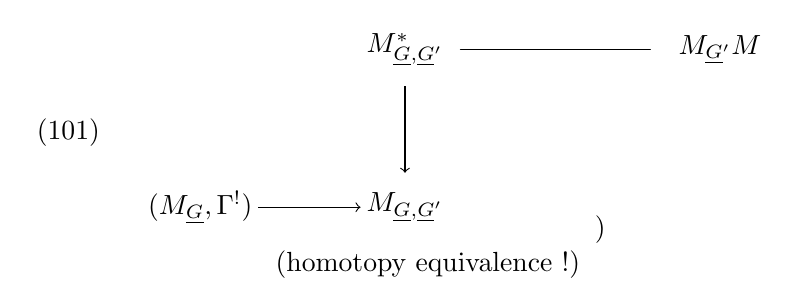
\begin{tikzpicture}[x=1cm,y=1cm]
\node[inner sep=2pt] (A) at (0,0) {$M^*_{\underline G,\underline G'}$};
\node[inner sep=2pt] (B) at (4,0) {$M_{\underline G'}\deleted{\unsure{M}}$};
\node[inner sep=2pt] (C) at (-2.6,-2) {$(M_{\underline G}\deleted{\unsure{,\Gamma^!}})$};
\node[inner sep=2pt] (D) at (0,-2) {$M_{\underline G,\underline G'}$};
\draw[line cap=round] ([xshift=4pt]A.east) -- ([xshift=-8pt]B.west);
\draw[->] ([yshift=-5pt]A.south) -- ([yshift=5pt]D.north);
\draw[->] (C.east) -- (D.west);
\node[anchor=east] at (-3.75,-1.05) {$(101)$};
\node[anchor=north west,inner sep=0pt] (caption) at (-1.65,-2.55) {(homotopy equivalence !)};
\node[anchor=base west,inner sep=0pt] at ([xshift=5pt,yshift=5pt]caption.north east) {$\unsure{)}$};
\end{tikzpicture}}
giving rise \unsure{to|:} morphisms of groupoids
\margin{78}
